\section{}\label{question4}

\subsection{}
We implement \verb policy_evaluation and \verb policy_improvement to run the \verb policy_itertation algorithm.

\verb policy_evaluation evaluates the update for value function at each state, according to Bellman equation.
\verb policy_improvement uses the \verb policy_evaluation to greedily choose the new action at each state.

Full code is attached. The result is shown in \ref{fig_op_det} (a).

\subsection{} 
We implement \verb value_iteration algorithm. We don't evaluate policy as before, instead we just select action that maximises the value function update according to Bellman equation. 

Full code is attached. The result is shown in \ref{fig_op_det} (b).

We also present computing time (code executed on our laptop) for comparison. Evidently, {\bfseries value iteration is significantly faster than policy iteration}, since in policy iteration we need to perform "policy evaluation" for each updated value function. Note that the optimal policy found in the end is the same for both cases, which assures us that the code is correct and both methods converge to the same optimal policy.

\begin{center}
\begin{tabular}{lclc}
(a) & 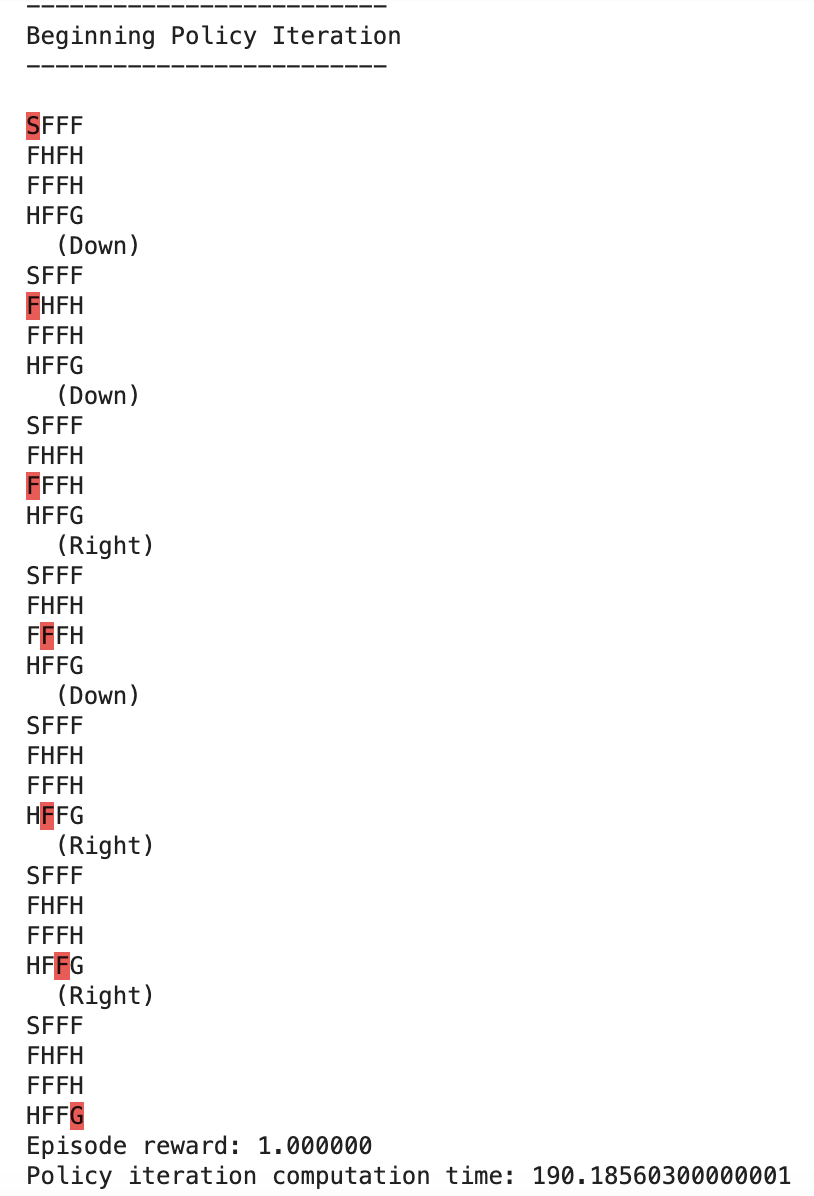
\includegraphics[width=7cm]{fig_pi_det.jpg} &
(b) & 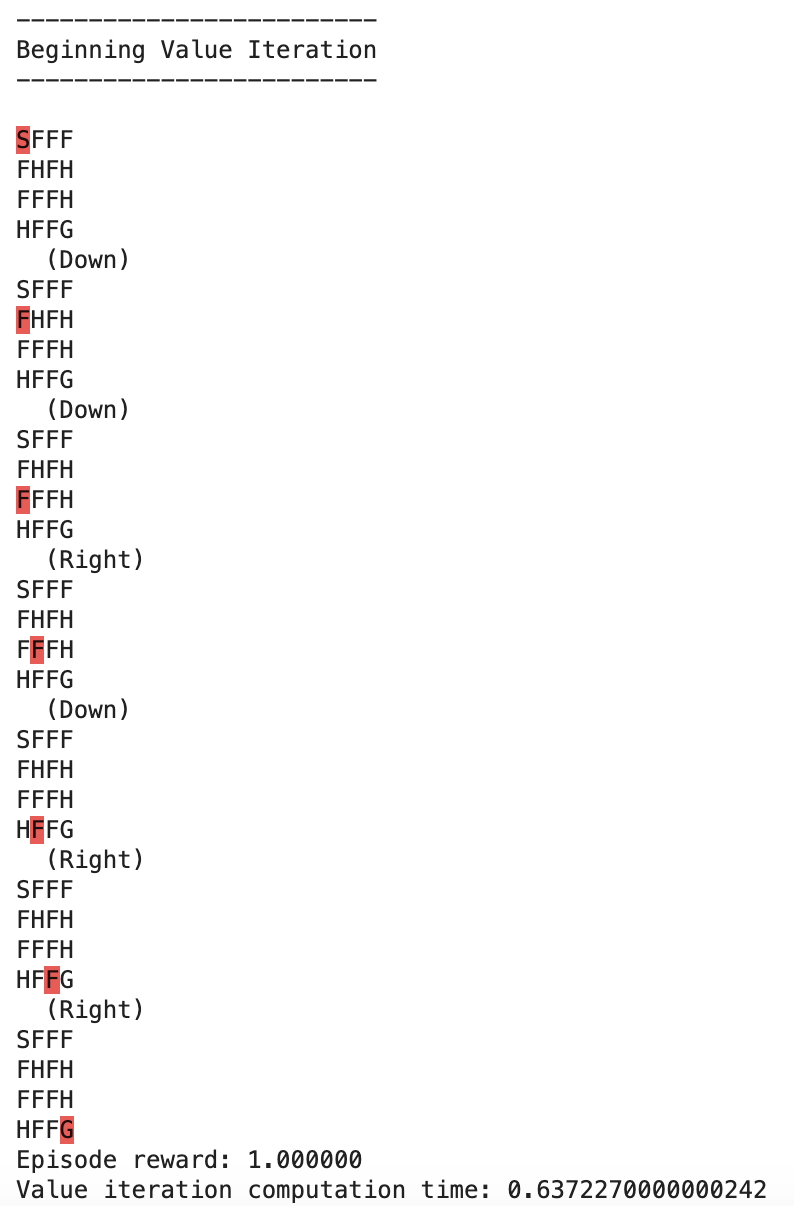
\includegraphics[width=7cm]{fig_vi_det.jpg} 
\end{tabular}
\captionof{figure}{Optimal policy found via (a) policy iteration and (b) value iteration. Below each table we present the computing time for comparison.}
\label{fig_op_det}
\end{center}


\subsection{}
We now re-run both value and policy iteration -based algorithm for the stochastic case (non-deterministic actions).

\begin{enumerate}
\item The value iteration: takes longer to converge and the optimal policy for stochastic case is different than in deterministic case (12 steps versus 7 steps).
\item The policy iteration: might not converge / needs much longer to converge. After the first run of 100 episodes it did not reach an optimal policy (ended up in a HOLE field instead of the target field). We re-ran it over 500 episodes for comparison and it did not converge either, hence we conclude it might either not converge at all, or do so asymptotically in which case computing the optimal policy is not computationally efficient.
\end{enumerate}

%\begin{center}
%\begin{tabular}{lclc}
%(a) & 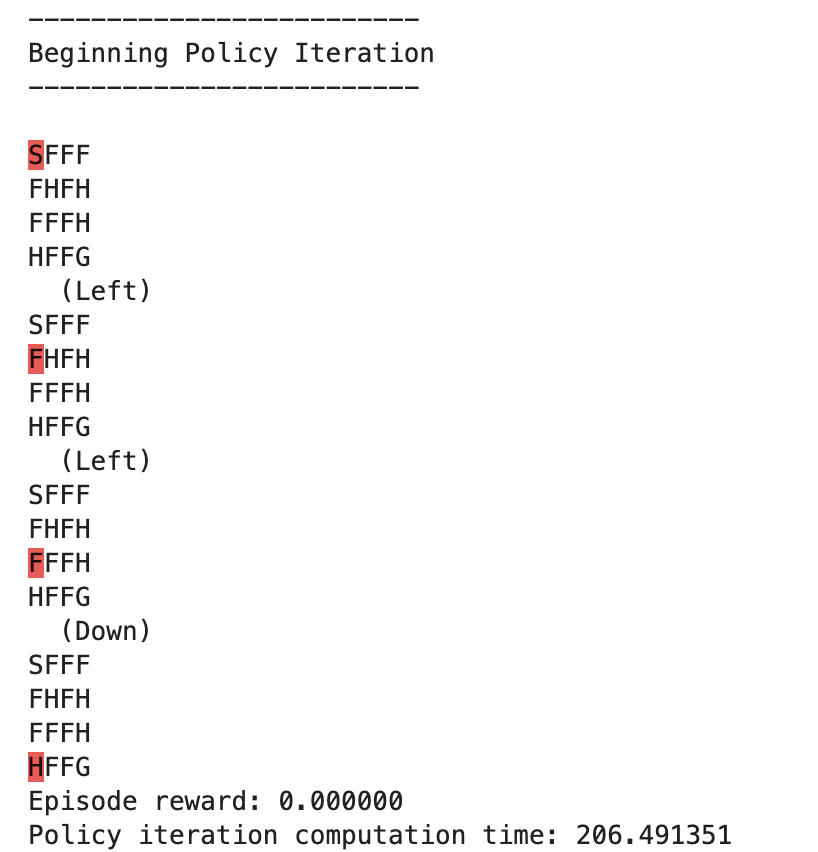
\includegraphics[width=7cm]{fig_pi_faulty.jpg} &
%(b) & \includegraphics[width=7cm]{fig_pi_sto.jpg} 
%\end{tabular}
%\captionof{figure}{Stochastic case, policy iteration:  (a) running over 100 episodes does not converge, (b) running over 200 episodes converges, albeit requires considerable computing time.}
%\label{fig_pi_sto}
%\end{center}
